\documentclass[12pt,letterpaper]{article}
\usepackage[utf8]{vietnam}
\usepackage{fullpage}
\usepackage[top=2cm, bottom=4.5cm, left=2.5cm, right=2.5cm]{geometry}
\usepackage{amsmath,amsthm,amsfonts,amssymb,amscd}
\usepackage{lastpage}
\usepackage{enumerate}
\usepackage{fancyhdr}
\usepackage{mathrsfs}
\usepackage{xcolor}
\usepackage{graphicx}
\usepackage{listings}
\usepackage{hyperref}
\hypersetup{%
  colorlinks=true,
  linkcolor=blue,
  linkbordercolor={0 0 1}
}
 
\renewcommand\lstlistingname{Algorithm}
\renewcommand\lstlistlistingname{Algorithms}
\def\lstlistingautorefname{Alg.}

\lstdefinestyle{Python}{
    language        = Python,
    frame           = lines, 
    basicstyle      = \footnotesize,
    keywordstyle    = \color{blue},
    stringstyle     = \color{green},
    commentstyle    = \color{red}\ttfamily
}

\setlength{\parindent}{0.0in}
\setlength{\parskip}{0.05in}

% Edit these as appropriate
\newcommand\course{MathAir2018}
\newcommand\hwnumber{}                  % <-- homework number
\newcommand\NetIDa{Nguyen Quang Huy}           % <-- NetID of person #1
\pagestyle{fancyplain}
\headheight 35pt
\lhead{\NetIDa}
\chead{\textbf{\Large Liner Regression \hwnumber}}
\rhead{\course \\ \today}
\lfoot{}
\cfoot{}
\rfoot{\small\thepage}
\headsep 1.5em

\begin{document}

\section*{Khái niệm Linear Regression}

    $\textbf{Bài toán Linear Regression là gì?}$
    
    Bài toán Linear Regression là bài toán đi tìm các hệ số tối ưu $w_1, w_2,.. w_0$ cho phương trình:
    
    $$ f(x) = w_0 + w_1*x_1 + w_2*x_2 + ... + w_n*x_n $$
    
    Ta đặt:
    
        $$
        \bar{\textbf{x}} 
        = 
        \begin{bmatrix}
        1 & x_1 & x_2 & x_3 & \dots  & x_n \\
        \end{bmatrix}
        $$
    
        $$
        \textbf{w} 
        = 
        \begin{bmatrix}
        w_0 \\ w_1 \\ w_2 \\ w_3 \\ \dots  \\ w_n 
        \end{bmatrix}
        $$
    
    Suy ra:
    
        $$
        y = f(x) 
        = 
        w_0 + w_1*x_1 + w_2*x_2 + ... + w_n*x_n 
        =
        \begin{bmatrix}
        1 & x_1 & x_2 & x_3 & \dots  & x_n \\
        \end{bmatrix}
        *
        \begin{bmatrix}
        w_0 \\ w_1 \\ w_2 \\ w_3 \\ \dots  \\ w_n 
        \end{bmatrix}
        = 
        \bar{\textbf{x}}*\textbf{w} 
        $$
    
    Từ đó dùng hệ số để dự đoán giá trị $\hat{y}$ với mỗi bộ dữ liệu $x_1', x_2',.. x_n'$
    
    

\section*{Cách giải bài toán}   

    Hệ số $w_1, w_2,.. w_0$ là tối ưu khi sự sai khác e của giá trị thực y và giá trị dự đoán $\hat{y}$ là nhỏ nhất (sai số dự đoán). Sai khác e được tính bằng công thức:
        
        $$
        \frac{1}{2} * e^2 
        = 
        \frac{1}{2} * (y - \hat{y})^2 
        = 
        \frac{1}{2} * (y - \bar{\textbf{x}}*\textbf{w})^2
        $$
        
    Như vậy với mỗi bộ dữ liệu $x_1, x_2,.. x_n $ và giá trị thực y ta lại có một sai khác e khác nhau, vậy để tối ưu ta cần tìm hệ số $w_1, w_2,.. w_0$ sao cho tổng sai khác giữa giá trị thực y và giá trị $\hat{y}$ của các bộ dữ liệu là nhỏ nhất, từ đấy ta đi đến khái niệm hàm mất mát:
        
        $$ 
        \mathcal{L}(\textbf{w}) 
        = 
        \frac{1}{2} * \sum_{i=1}^N (y_i - \bar{\textbf{x}}_i*\textbf{w})^2 
        $$
        
    Nếu ta đặt:
    
        $$
        \textbf{y} 
        =
        \begin{bmatrix}
        y_1 \\ y_2 \\ y_3 \\ \dots  \\ y_n \\
        \end{bmatrix}
        $$
    
    và
    
        $$
        \bar{\textbf{X}} 
        =  
        \begin{bmatrix}
        \bar{x}_1 \\ 
        \bar{x}_2 \\
        \bar{x}_3 \\ 
        \dots  \\ 
        \bar{x}_n \\
        \end{bmatrix}
        = 
        \begin{bmatrix}
        1 & x_{1 1} & x_{1 2} & \dots & x_{1 n} \\
        1 & x_{2 1} & x_{2 2} & \dots & x_{2 n} \\
        1 & x_{3 1} & x_{3 2} & \dots & x_{3 n} \\
        \dots & \dots & \dots & \dots & \dots & \\
        1 & x_{n 1} & x_{n 2} & \dots & x_{n n} \\
        \end{bmatrix}
        $$
        
    thì tích : $\bar{\textbf{X}}*\textbf{w}$ sẽ có dạng:
        
        $$
        \begin{bmatrix}
        1 & x_{1 1} & x_{1 2} & \dots & x_{1 n} \\
        1 & x_{2 1} & x_{2 2} & \dots & x_{2 n} \\
        1 & x_{3 1} & x_{3 2} & \dots & x_{3 n} \\
        \dots & \dots & \dots & \dots & \dots & \\
        1 & x_{n 1} & x_{n 2} & \dots & x_{n n} \\
        \end{bmatrix}
        *
        \begin{bmatrix}
        w_0 \\ w_1 \\ w_2 \\ \dots  \\ w_n \\
        \end{bmatrix}
        =
        \begin{bmatrix}
        w_0 + w_1 * x_{1 1} + w_2 * x_{1 2} + \dots + w_n * x_{1 n}\\
        w_0 + w_1 * x_{2 1} + w_2 * x_{2 2} + \dots + w_n * x_{2 n}\\
        w_0 + w_1 * x_{3 1} + w_2 * x_{3 2} + \dots + w_n * x_{3 n}\\
        \dots \\
        w_0 + w_1 * x_{n 1} + w_2 * x_{n 2} + \dots + w_n * x_{n n}\\
        \end{bmatrix}
        =
        \begin{bmatrix}
        \bar{\textbf{x}}_1*\textbf{w} \\
        \bar{\textbf{x}}_2*\textbf{w} \\ 
        \bar{\textbf{x}}_3*\textbf{w} \\
        \dots \\  
        \bar{\textbf{x}}_n*\textbf{w}
        \end{bmatrix}
        $$
        
    và hiệu $\textbf{y} - \bar{\textbf{X}}*\textbf{w}$ sẽ bằng:
        
        $$
        \begin{bmatrix}
        y_1 - \bar{\textbf{x}}_1*\textbf{w} \\ 
        y_2 - \bar{\textbf{x}}_2*\textbf{w} \\ 
        y_3 - \bar{\textbf{x}}_3*\textbf{w} \\ 
        \dots  \\ 
        y_n - \bar{\textbf{x}}_n*\textbf{w} \\
        \end{bmatrix}
        $$
        
    Như vậy có thể viết gọn $\mathcal{L}(\textbf{w})$ như sau:
        
        $$
        \mathcal{L}(\textbf{w}) 
        = 
        \frac{1}{2} * 
        \lVert 
            \textbf{y} - \bar{\textbf{X}}*\textbf{w}
        \rVert_2^2
        $$
    
    $ \textbf{Để giải bài toán tối ưu, ta cần tìm nghiệm bằng 0 của đạo hàm của hàm mất mát: } $
        $$
            \mathcal{L}'(\textbf{w}) = \sum_{i=1}^N (\frac{1}{2} (y_i - \bar{\textbf{x}}_i*\textbf{w})^2)'
        $$
        $$
            = \sum_{i=1}^N  \frac{1}{2} * 2(y_i - \bar{\textbf{x}}_i*\textbf{w}) * (y_i - \bar{\textbf{x}}_i*\textbf{w})' 
        $$
        $$
            = \sum_{i=1}^N  (y_i - \bar{\textbf{x}}_i*\textbf{w}) * -(\bar{\textbf{x}}_i * \textbf{w})'
        $$
        $$
            = \sum_{i=1}^N  (y_i - \bar{\textbf{x}}_i*\textbf{w}) * -( \bar{\textbf{x}_i}^T)
        $$
        $$
            = \sum_{i=1}^N  (y_i - \bar{\textbf{x}}_i*\textbf{w}) * -( \bar{\textbf{x}}_i^T)
        $$
        $$
            = \sum_{i=1}^N  (\bar{\textbf{x}}_i*\textbf{w} - y_i) * \bar{\textbf{x}_i^T}
        $$
        $$
            = \bar{\textbf{X}}^T * (\bar{\textbf{X}}\textbf{w} - \textbf{y})
        $$
        $$
            = \bar{\textbf{X}}^T * \bar{\textbf{X}}\textbf{w} - \bar{\textbf{X}}^T * \textbf{y}
        $$
    như vậy phương trình bằng 0 tương đương với
        $$
            \bar{\textbf{X}}^T * \bar{\textbf{X}}\textbf{w} = \bar{\textbf{X}}^T * \textbf{y}
        $$
    TH1: ma trận $\bar{\textbf{X}}^T * \bar{\textbf{X}}$ là khả nghịch, suy ra:
        $$
            (\bar{\textbf{X}}^T * \bar{\textbf{X}}) ^{-1} * \bar{\textbf{X}}^T * \bar{\textbf{X}} * \textbf{w} = (\bar{\textbf{X}}^T * \bar{\textbf{X}}) ^{-1} * \bar{\textbf{X}}^T * \textbf{y}
        $$
    suy ra:
        $$
             \textbf{w} = \bar{\textbf{X}}^T * \bar{\textbf{X}}) ^{-1} * \bar{\textbf{X}}^T * \textbf{y}
        $$
    
    TH2: ma trận $\bar{\textbf{X}}^T * \bar{\textbf{X}}$ là không khả nghịch thì:
        $$
            \textbf{w} = (\bar{\textbf{X}}^T * \bar{\textbf{X}}) ^{\dagger} * \bar{\textbf{X}}^T * \textbf{y}
        $$

\section*{Code trong python}
\begin{enumerate}
    \item \textbf {Đặt bài toán thực tế}
    \\
    Anh X đang chuẩn bị ứng tuyển vào công ty A và muốn xem liệu anh nên yêu cầu mức lương bao nhiêu. Là một người trẻ mới có kinh nghiệm x năm trong nghề và ra trường với bằng giỏi, anh X không muốn yêu cầu mức lương cao quá để bị từ chối cũng như không muốn một mức lương quá thấp so với năng lực của mình. 
    \\
    Nhờ quen biết anh đã xin được bảng lương của mọi người trong công ty cùng số năm kinh nghiệm, trình độ đại học của mỗi người trong nghề.
    \\
    Dữ liệu có thể xem tại \href{https://github.com/LittleCuteBug/LinearReagression/blob/master/Salary_Data.csv}{đây}
    \\
    Ta có thể giả định số năm trong nghề và tấm bằng sau khi ra trường sẽ tỷ lệ thuận với mức lương nhận được, từ đó ta có thể tạo bài toán
    $$
        f(x) = w_0 + w_1 * a + w_2 * b
    $$
    trong đó :
    \begin{enumerate}
        \item f(x) là mức lương nhận được
        \item a là số năm kinh nghiệm
        \item b là mức bằng đại học, ở đây ta biểu diễn (bằng trung bình, bằng khá, bằng giỏi) bằng (1,2,3)
    \end{enumerate}
    \item \textbf {Python code}
    \\
    Xử lý dữ liệu:
    \begin{figure}[ht]
        \centering 
        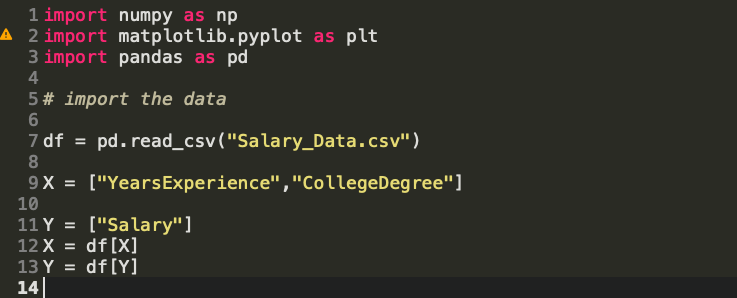
\includegraphics[scale=0.5]{python1.png}
    \end{figure}
    \\
    \\
    Áp dụng công thức để tính toán tìm hệ số w tối ưu:
    \begin{figure}
        \centering 
        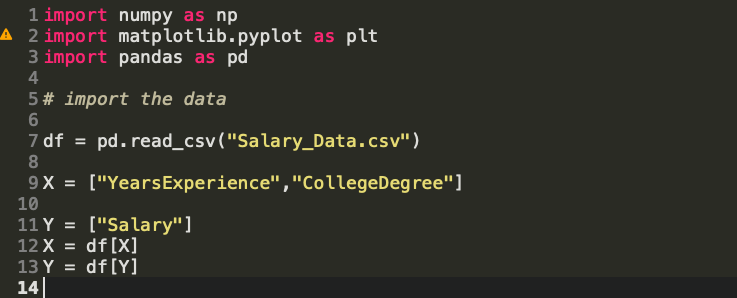
\includegraphics[scale=0.5]{python1.png}
    \end{figure}
    \\
    \\
    \\
    \\
    \\
    \\
    \\
    Từ đó ta tính được bộ dữ liệu w bằng \textbf{[15413,10050.8,4491.8]}
    \item \textbf {Kết quả}
    \\
    Vậy từ đó anh X có thể đánh giá mức lương của mình theo công thức để đề nghị mức lương hợp lý:
    $$
        f(x) = 15413 + 10050.8 * \textit{số năm kinh nghiệm} + 4491.8 * \textit{mức bằng đại học}
    $$
    ví dụ anh T có 3 năm kinh nghiệm và bằng đại học mức khá, khi được tuyển vào công ty A anh T sẽ có thể dự đoán mức lương xấp xỉ bằng:
    $$
        f(x) = 15413 + 10050.8 * 3 + 4491.8 * 2 = 54549
    $$
    
\end{enumerate}
\section*{Nhận xét thuật toán}
Ta có thể thấy Linear Regression là một thuật toán ngắn gọn và dễ dàng cài đặt, mặc dù độ chính xác có thể dễ sai lệch khi có bộ dữ liệu chưa tốt: có một số dữ liệu sai khác quá lớn với các dữ liệu khác (ví dụ trong bộ dữ liệu phía trên nếu có nhân viên lương quá cao trong khi không có kinh nghiệm gì và bằng thấp)
\end{document}
